
% \begin{itemize}
% \item FEM description e.g. ODC mount FEM, M1 FEM, frequency range, ...
% \item pretty pictures of the whole FEM and the top-end + ASMS part
% \item ...
% \end{itemize}

The finite element mesh of the telescope is the basis of a linear state space model that utilizes modal and static solutions of the FEM. Modes are obtained from 0 to 1475 Hz. 
To reduce the number of modes to a manageable number a constraint is added when solving for modes above 75 Hz The constraint fixes all nodes below the truss interface of the topend. 
The static solution is employed to correct the DC gain of the state space model which is due to omitting higher frequency modes as well as the additional constraint.

ASM cells and corresponding cabinets are attached to the top-end frame. 
The ASM is current as of June 2021.
The ASM mesh features flexible facesheets held in place by flexures around its rim. 
To actuate the facesheet and to simulate wind disturbance forces and moments may be applied which are spread via an interpolation element (RBE3). 
In the case of actuation equal and opposite reactions are applied to the cold plate. Similarly forces may be applied between the reference body and the facesheet to simulate fluid damping. The voice coil actuators are not explicitly modeled to avoid a large number of extra modes. 
The ASM cells may be positioned by changing the lengths of the positioners via axial forces.

The mount is current as of April 2021, and the configuration is 0 deg azimuth and 30 deg zenith. 
The mount is ``unlocked'', such that the  azimuth, elevation and GIR rotation angles can be controlled via feedback controllers utilizing drives and encoders.
 
M1 segments are explicitly modeled in detail, including honeycomb and load spreaders. 
M1 pneumatic actuators are implemented as forces applied to load spreaders on the back surface of the M1 segments with reaction forces applied to the top-plate of the M1 segments. 
The M1 segments may be positioned by changing the length of the hardpoints (rod elements) via axial forces.

The pier mesh is the mesh used by the mount vendor as of June 2021. It is not the model currently generated by IDOM.

It would be easy to have errors in the setup of the FE model, for example forces applied to the wrong node. 
To reduce the likelihood of such errors extensive (but not exhaustive) tests validate the inputs and outputs of the model. 
For example one automated check tests that the mirror segments move as expected for given inputs to the hardpoints and positioners.
The current test suite covers the positioning of M1 and M2 segments, mount
drives and encoders as well as some more general stiffness tests, but not the
active optics on M1 and M2.

\begin{figure}
  \centering
  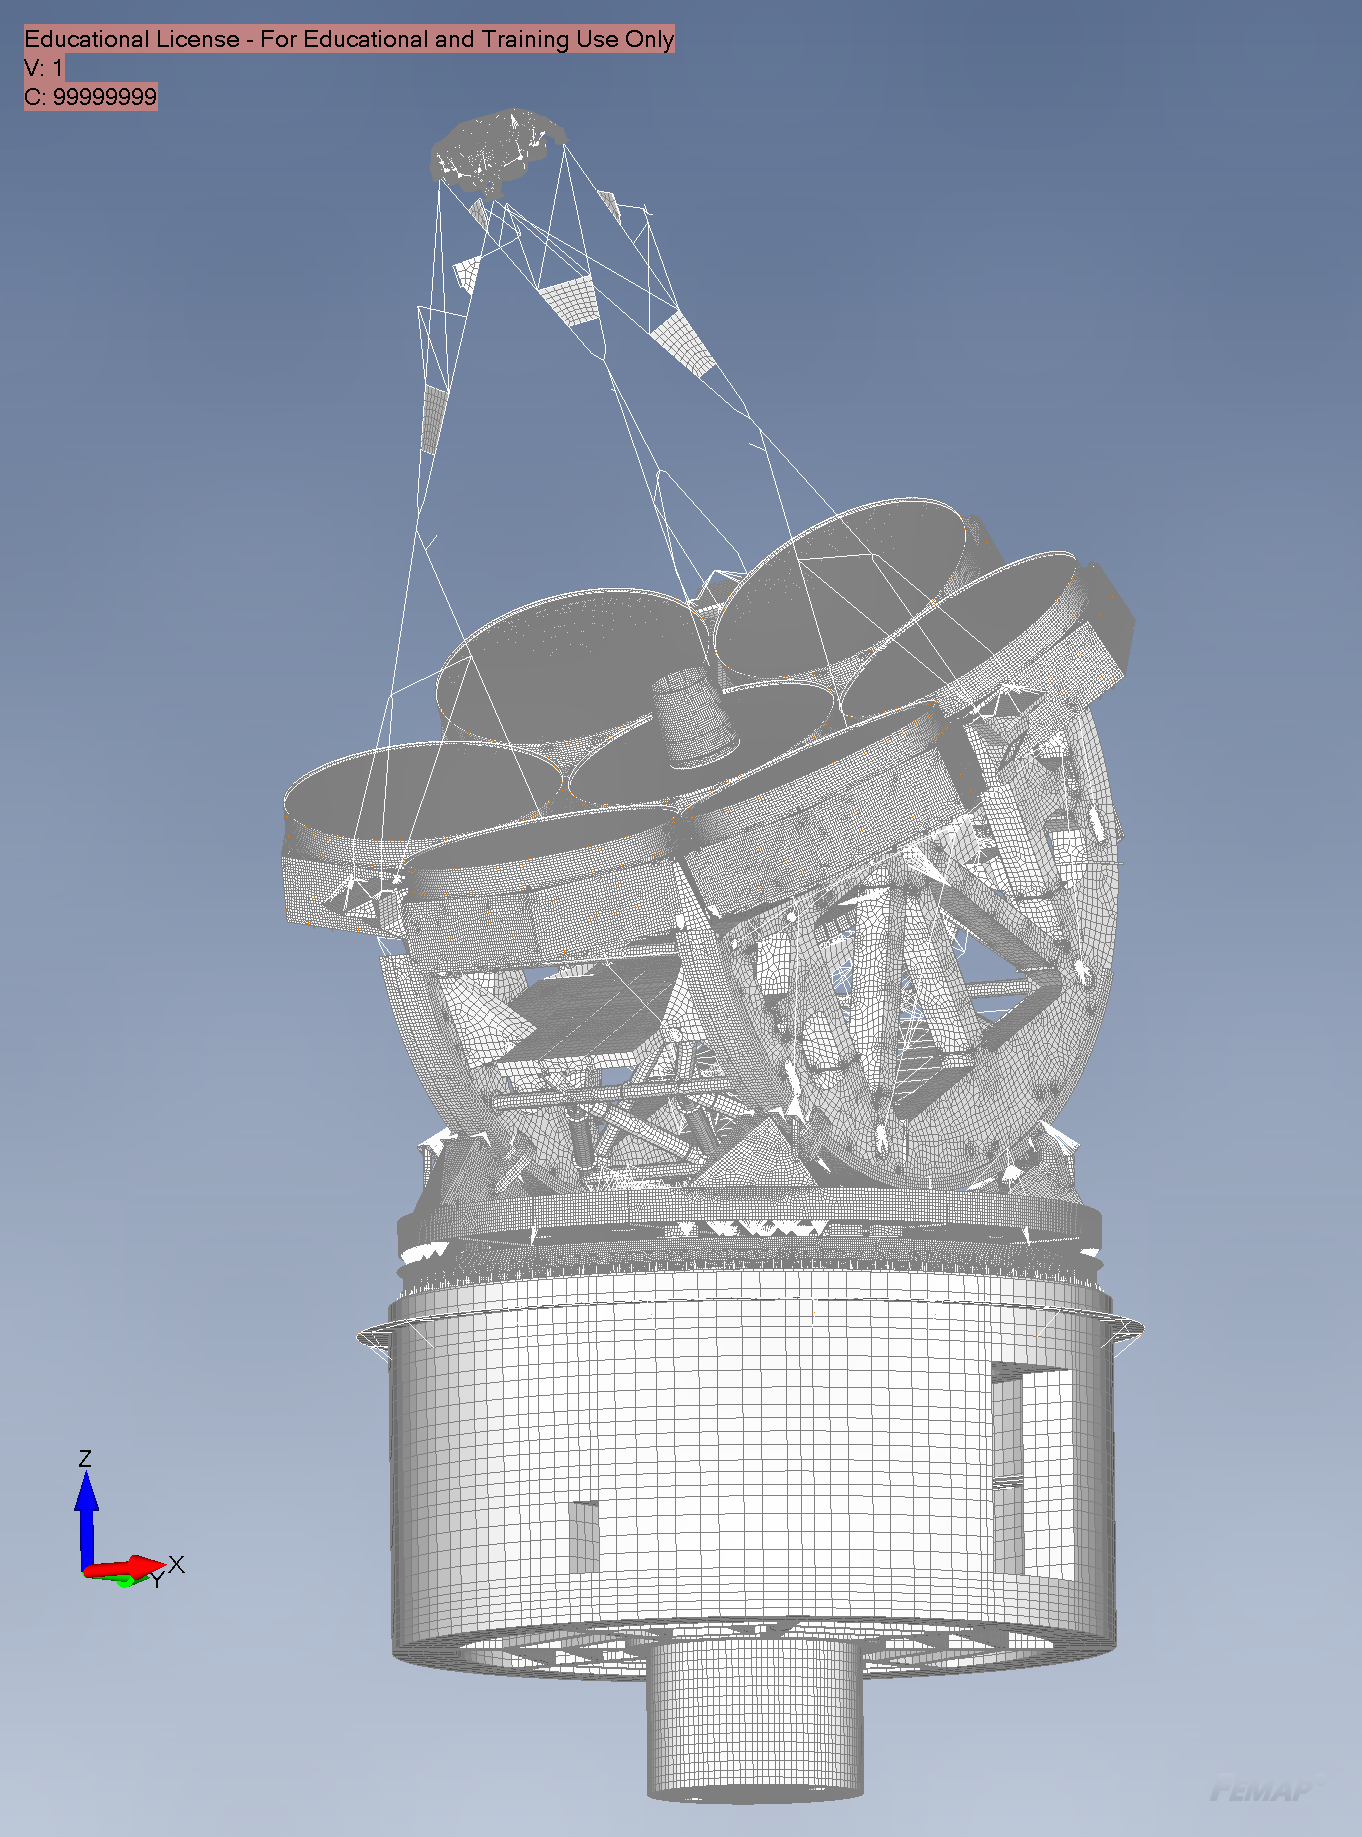
\includegraphics[width=0.5\textwidth]{FEM/whole_telescope.png}
  \caption{Whole telescope FEM.}
  \label{fig:fem-whole}
\end{figure}

\begin{figure}
  \centering
  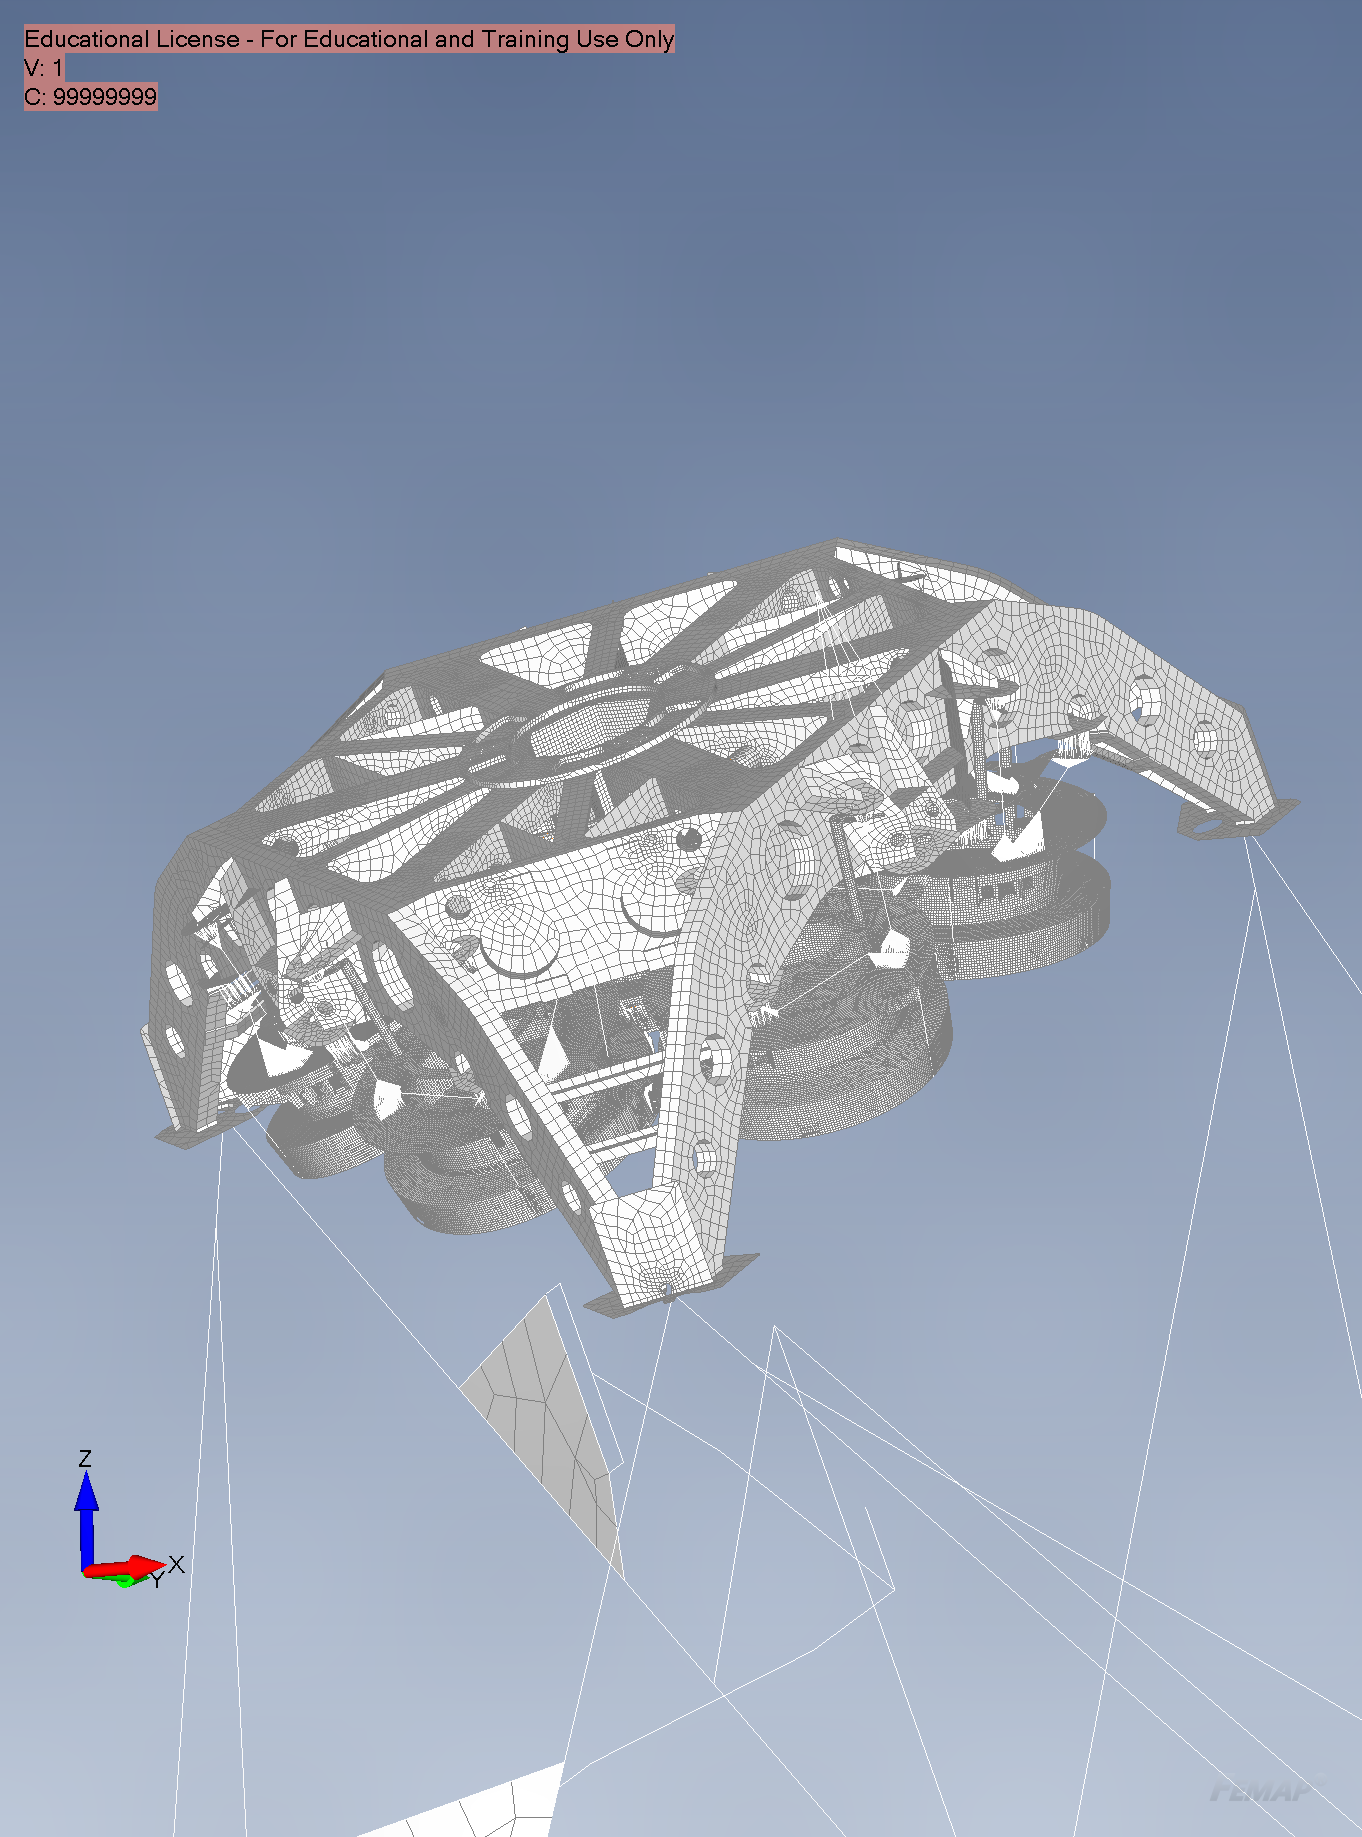
\includegraphics[width=0.6\textwidth]{FEM/topend.png}
  \caption{Top-end FEM detail.}
  \label{fig:fem-topend}
\end{figure}

\begin{figure}
  \centering
  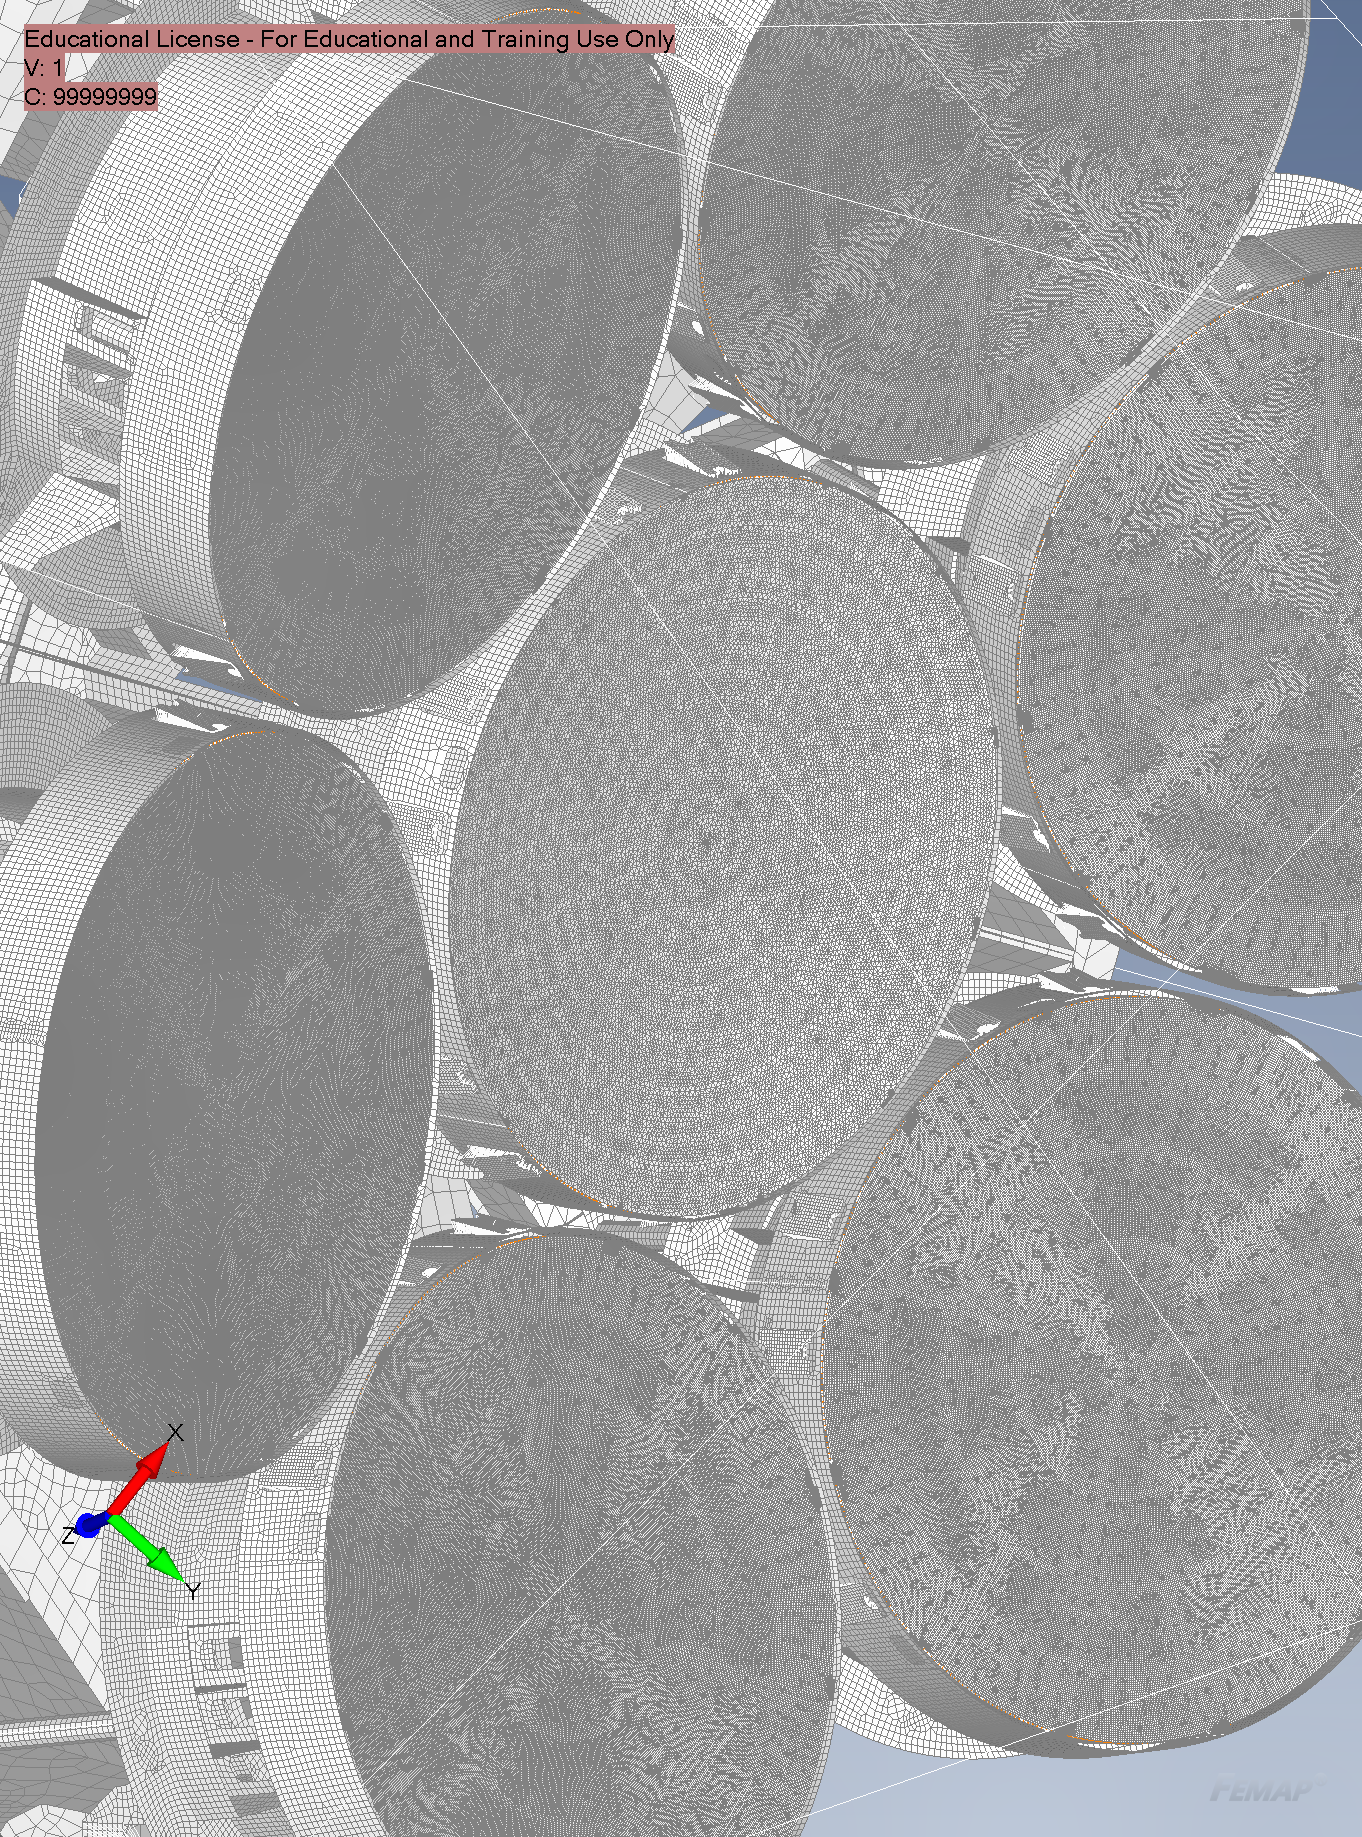
\includegraphics[width=0.6\textwidth]{FEM/facesheets.png}
  \caption{Facesheets FEM detail.}
  \label{fig:fem-facesheets}
\end{figure}

%%% Local Variables:
%%% mode: latex
%%% TeX-master: "asm-im"
%%% End:
